\documentclass[aspectratio=169]{beamer}              % only frames

% for themes, etc.
\mode<presentation>
\usetheme{Madrid} 
\usecolortheme{crane}

%\usepackage{times}  % fonts are up to you
% The usual suspects
\usepackage{multirow, booktabs, dcolumn, color, graphicx} % Tables\usepackage{graphicx}
\usepackage{amsmath,amssymb,amsthm}
% Strikethrough text
\usepackage{soul}
% Adjust box to fit tabulars
\usepackage{adjustbox}
% Embed video
\usepackage{media9}
% For notes
\usepackage{pgfpages}
\setbeameroption{hide notes} % Only slides
%\setbeameroption{show only notes} % Only notes
%\setbeameroption{show notes on second screen=right} % Both
% Give a slight yellow tint to the notes page
%\setbeamertemplate{note page}{\pagecolor{yellow!5}\insertnote}\usepackage{palatino}
% Use colors by name
\usepackage{xcolor}
% EMBEDDING VIDEO IS POSSIBLE WITH PDFPC USE PDF PC to present
\usepackage{multimedia}



% The table highlighting for hypothesis discussion.
\usepackage[beamer,customcolors]{hf-tikz}
\usetikzlibrary{calc}

% To use background images
\newenvironment{colorframe}[2][]{%
\setbeamercolor{background canvas}{bg=#1}
\begin{frame}\color{white}}
{\end{frame}}


% To set the hypothesis highlighting boxes red.
\tikzset{hl/.style={
    set fill color=red!80!black!40,
    set border color=red!80!black,
  },
}

% Set Graphics folder
\graphicspath{{./figures/}}


% these will be used later in the title page
\title{Surveillance Online}
\subtitle{The Case for Privacy}
\author{Irfan Kanat}
\institute[CBS]{{Department of Digitization}\\ Copenhagen Business School}
\date{\today}



\begin{document}

% this prints title, author etc. info from above
\begin{frame}

	\titlepage

	\vfill
	{\tiny \centering This work is licensed under a \href{http://creativecommons.org/licenses/by/4.0/}{Creative Commons Attribution 4.0 International License}.}

\end{frame}

\note{In this module we will talk about government surveillance.}



\begin{frame}
	\frametitle{Who is Tracking You?}

	Other people	\vspace{1em}    

	Businesses \vspace{1em}

	\textbf{Governments}	\vspace{.5em}

	\hspace{1em} Mass Surveillance

	\hspace{1em} Targetted Surveillance \vspace{1em}

\end{frame}

\note{We talk about other people tracking you online in Cyberbullying module. We talk about private companies tracking you in the Product is You module.

Our focus on this module is the Government surveillance.}


\begin{frame}
	\frametitle{Snowden Revelations}
    
	\centering

    \only<1>{

    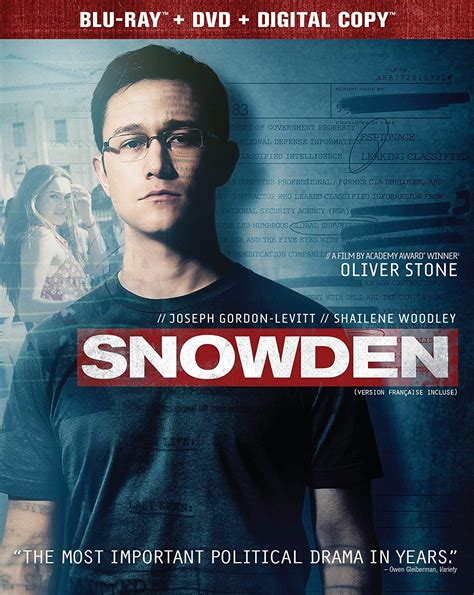
\includegraphics[width = \textwidth, height = .85\textheight, keepaspectratio]{figures/Snowden.jpeg} \hspace{1em}
    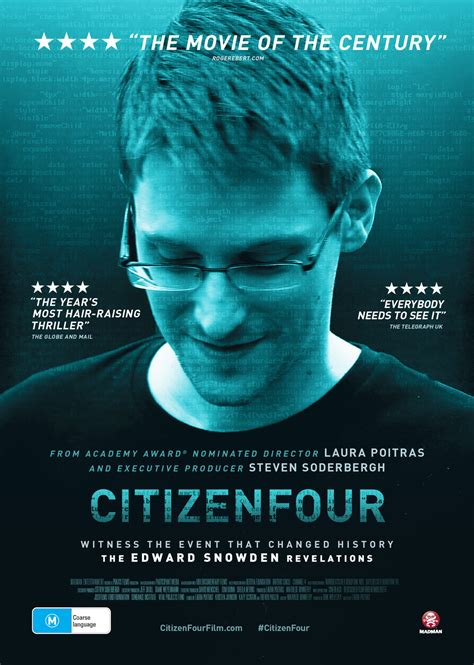
\includegraphics[width = \textwidth, height = .85\textheight, keepaspectratio]{figures/citizen4.jpeg}

    }

\end{frame}

\note{In 2013, the world became aware of the extend of American surveillance capabilities through a series of leaks published in the Guardian and the WaPo. The leaks revealed that the inteligence agencies have gone beyond their legal mandate, and violated the US constitution (court ruling in 2020). This was such big news, that hollywood made a movie about it. They cast Joseph Gordon-Levitt as Snowden and Oliver Stone directed the movie. Nicolas Cage is even in it.

It is an exciting piece of thriller, that glosses over the scandal a bit. It is after all a movie and not a documentary. If you are truly interested, I recommend you watch the documentary Citizen 4. It is available for free on the internet \url{https://www.youtube.com/watch?v=EDhB-A23IUk}. You can see actual footage of Snowden talking to the director of the documentary and journalists from the Guardian and WaPo. It is the actual footage before the revelations. }


\begin{frame}
	\frametitle{Snowden Revelations}
	\framesubtitle{What were they?}

\begin{itemize}
	\item Stellar Wind (SSO): Phone Records
	\item Prism: American Companies
	\item XKeyscore: Record of Online Activity
	\item Backdoors to Tech Giants
	\item Undermining Encryption
\end{itemize}
	
\end{frame}

\note{The full extent of the revelations is too much to cover in a short video. I will focus on some of the most relevant cases for our topic.

(1) All american phone companies were sharing phone records (who called whom, when) with NSA. Millions of American Citizens' information was shared with **secret** court orders. The court orders were broad and allowed NSA to collect information on thousands of unrelated citizens for each foreign suspect they were interested in. This is a big deal as normally spying on American citizens is legally more complex. (2) Through a program known as PRISM, NSA could compel American companies to give NSA access to their records. Google, Apple, Facebook... All of these companies were sharing information with NSA and were not allowed to speak of it. (3) XKeyscore program allowed NSA to access records of your online activity. The records included browsing history, searches, emails, chats, metadata. NSA training materials promoted the program as covering "nearly everything a typical user does on the Internet." What was the most shocking was, this program did not require prior authorization. NSA could tap into this information without a warrant, or a court clearance. (4) NSA tried to undermine encryption. (5) PRISM required some tiny legal hurdle. When NSA couldn't get what they wanted through PRISM, they went through their backdoors into links between American tech giants datacenters directly.

American's had legal protections agains government surveilance. A lot of these efforts violated those protections. 

The vast scope of the surveilance aparatus would have made the Eastern Germany salivate. Thanks to technology, US was able to scale spying to much greater extend than authoritarian soviet states ever could.}


\begin{frame}
	\frametitle{NSA and Surveillance . . . Made Simple}

	\centering

    \movie{
\includegraphics[width = \textwidth, height = .8\textheight, keepaspectratio]{figures/guardian.png}}{figures/guardian.mp4}
    
    {\tiny \href{https://www.youtube.com/watch?v=GoM4jIZbTtQ}{The Guardian}}

\end{frame}

\note{Guardian, the original newspaper that released the story made a neat animation that explains what is going on.

\url{https://www.youtube.com/watch?v=GoM4jIZbTtQ}}


\begin{frame}
	\frametitle{Surveilance Is Not Just an American Problem}
    
	\only<1>{
		\begin{quote}{§ 72}\\
			Boligen er ukrænkelig. Husundersøgelser, beslaglæggelse og undersøgelse af breve og andre papirer samt brud på post-, telegraf- og telefonhemmeligheden må, hvor ingen lov hjemler en særegen undtaglse, alene ske efter en retskendelse. 
		\end{quote}
	}

	\only<2>{
		\centering

		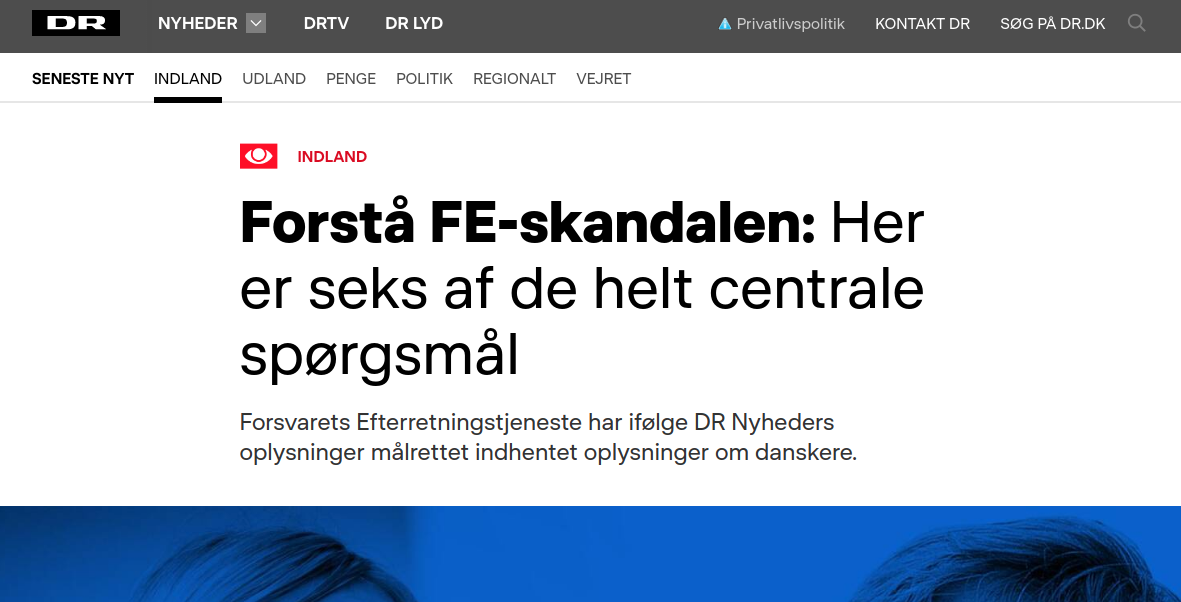
\includegraphics[width = \textwidth, height = .85\textheight, keepaspectratio]{figures/FE-Skandalen.png}
	}

\end{frame}

\note{Danes can expect the government to respect their privacy as it is enshrined in the 72nd article of the Danish constitution and the laws based on this. 

Yet Denmark too had its share of intelligence faux pas. Since 2014, there have been revelation after revelation about FE's illegal collaboration with NSA almost every year. Yet somehow nothing seems to change. The spy agencies prevented by law from violating their citizens' privacy rely on each other to spy on their citizens and share the information in the cases that require the most eggregious violations of the laws.}

\begin{frame}
	\frametitle{But I Have Nothing to Hide!}

	\centering
    
    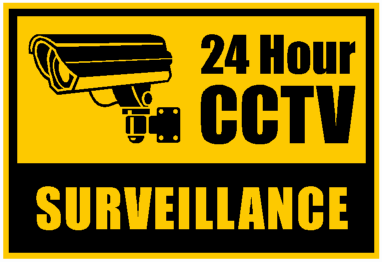
\includegraphics[width = \textwidth, height = .85\textheight, keepaspectratio]{figures/cctv-surveillance.png}

\end{frame}

\note{
	Obviously as with every topic worth consideration, there is a spectrum of views with regards to government surveillance. It is not a binary decision, where one has to opt for full surveilance or no surveillance. It is a spectrum and what you are comfortable with the government knowing will place you somewhere in between the two extremes.

	The most common argument against privacy has been ``If you have nothing to hide, you have nothing to fear.''

	The argument is that citizens should be willing to sacrifice some of their privacy in exchange for the security of the society.}

\begin{frame}
	\frametitle{But I Have Nothing to Hide!}
    
    \begin{quote}
    	``Arguing that you don't care about the right to privacy because you have nothing to hide is no different than saying you don't care about free speech because you have nothing to say.''	
    \end{quote}
	\hfill Edward Snowden \hspace{2em}

\end{frame}

\note{
	The counter point is that the trade off is not so much a security-privacy trade off, as it is a control-liberty trade off. 

	A right (such as given to citizens by the constitution) does not require the citizen to justify using it. It is the government that needs to justify the violation of it.

	As Snowden succintly put: ``Arguing that you don't care about the right to privacy because you have nothing to hide is no different than saying you don't care about free speech because you have nothing to say.''


	I would like to point out a few other angles:

	1- What your government considers illegal can change.

	2- Without breaking the rules, the society does not progress. Many things we consider natural today were illegal in the past (interracial marriage, same sex relations, race equality). Only through society being able to violate the laws were we able to reform our laws to match our society. With online surveillance we are entering an era of unprecedented surveilance capability. In this new system, the government is able to police 100\% of infractions. Meaning, if strictly enforced, the laws can stagnate.
}

\begin{frame}
	\frametitle{What can a Citizen Do?}

	\begin{itemize}
		\item Use your political rights.
		\item Harden your security.
			\begin{itemize}
				\item Make it harder to link your data
				\item Use encryption
				\item Use a VPN
			\end{itemize}
	\end{itemize}

	\only<2>{With regards to targeted surveillance\ldots Just give up.}

\end{frame}

\note{
Against mass surveillance: No matter what you believe in about surveillance. No matter if you believe every one should be under constant surveillance 24/7 or that government should never surveil any one ever. Make sure to make your voice heard. Use your political rights: vote, write to your representatives, and protest. 

If you are worried about being caught in a mass surveillance dragnet. Use encryption, make yourself a harder target. Take precautions to prevent linking of your data (credit card, transport pass, cell phone, email, etc.).

Against targeted surveillance: As Mickens puts it... If Mossad wants to do Mossady things, you will get Mossaded upon. You can ditch your electronics, move into a submarine and live in the middle of the ocean. You will still get Mossaded upon.}



\end{document}
